\section{Bonus}
\subsection{Compare the Results in terms of target dataset \& CNN model}
We gathere terminal output windows for the comparison results.\\
\vspace{-4mm}
\begin{figure}[h!]
\centering
\subfloat[Given Data \& Given Model , \textbf{Test Accuracy : 84.853} ]{
    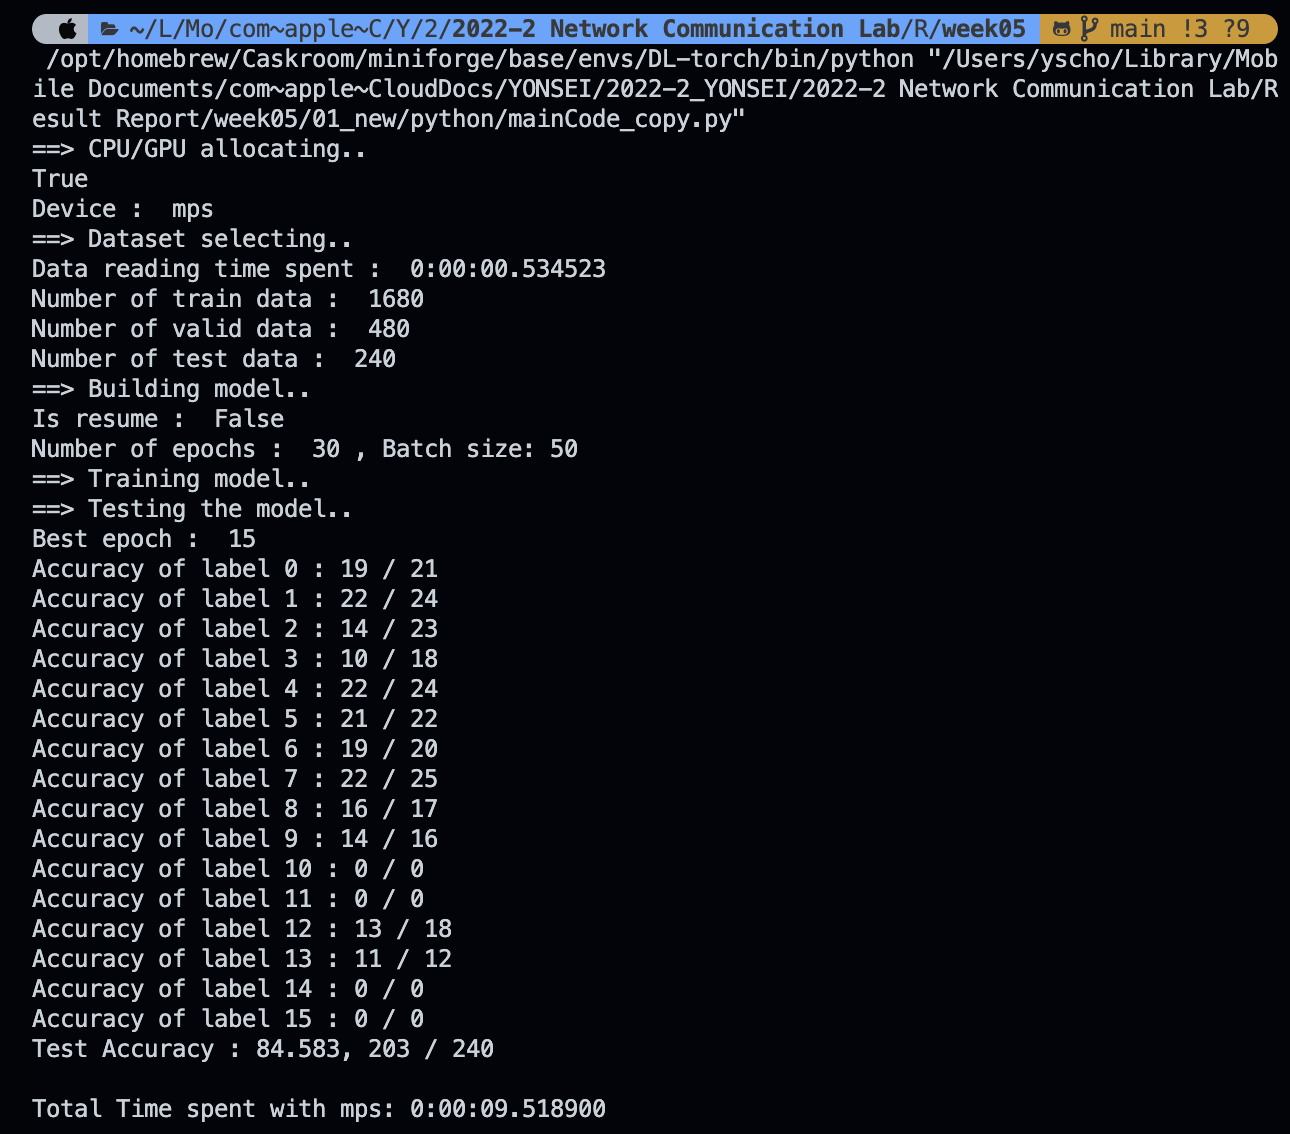
\includegraphics[width=0.48\textwidth]{image/week05/4-2-1.png}
}
\subfloat[Custom Data \& Given Model , \textbf{Test Accuracy : 89.474}]{
    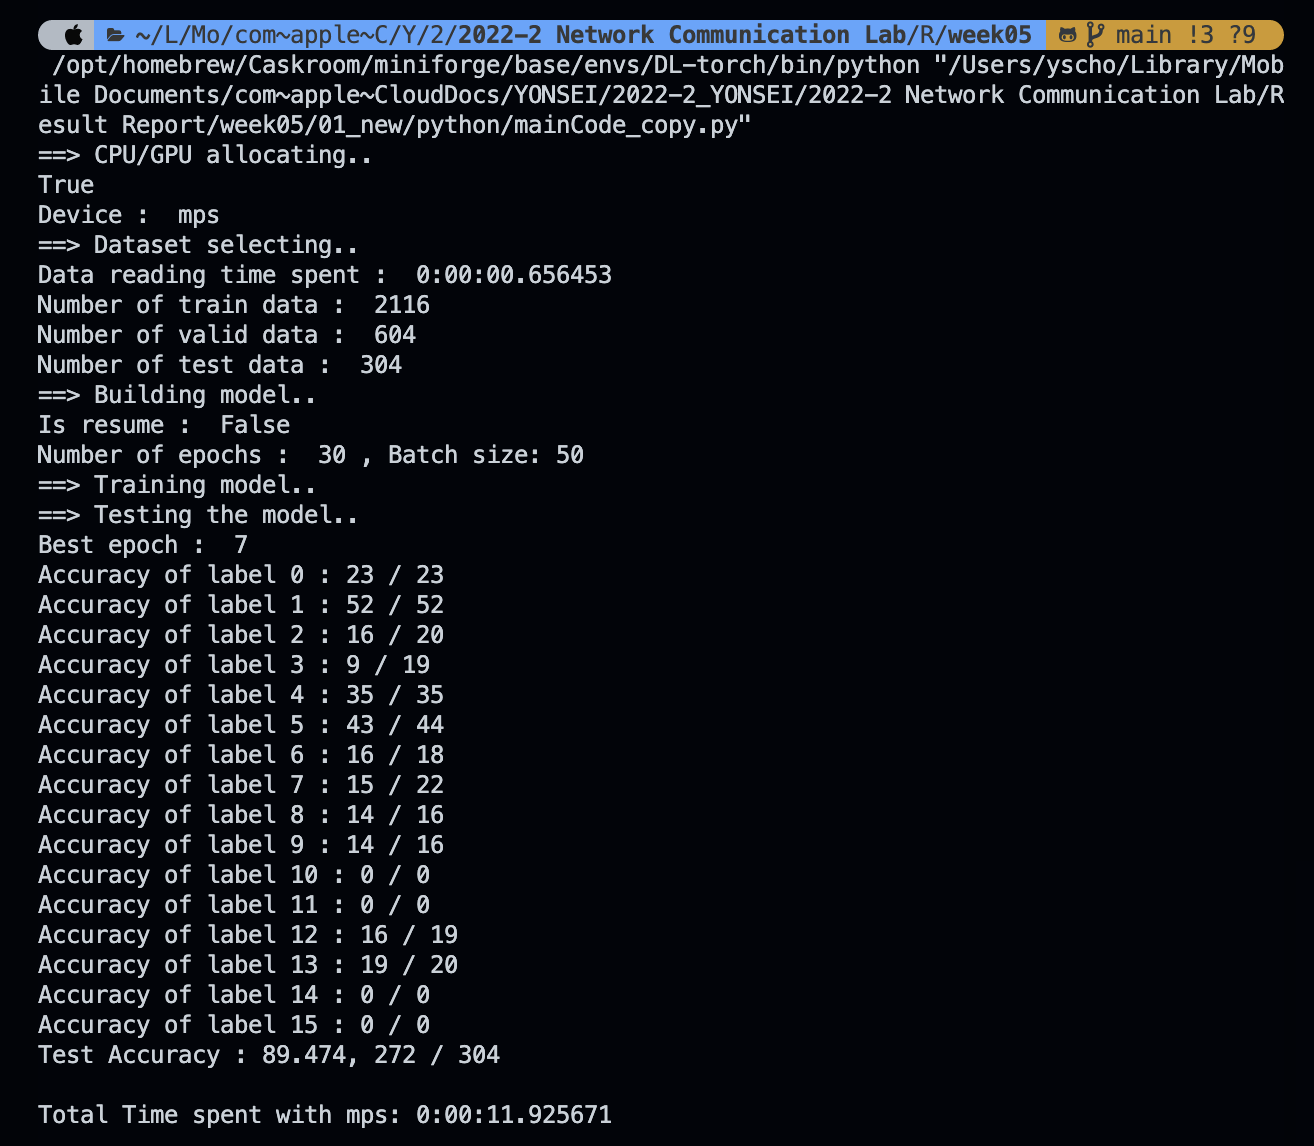
\includegraphics[width=0.48\textwidth]{image/week05/4-2-2.png}
}
\hfill
\subfloat[Given Data \& Custom Model , \textbf{Test Accuracy : 92.500}]{
    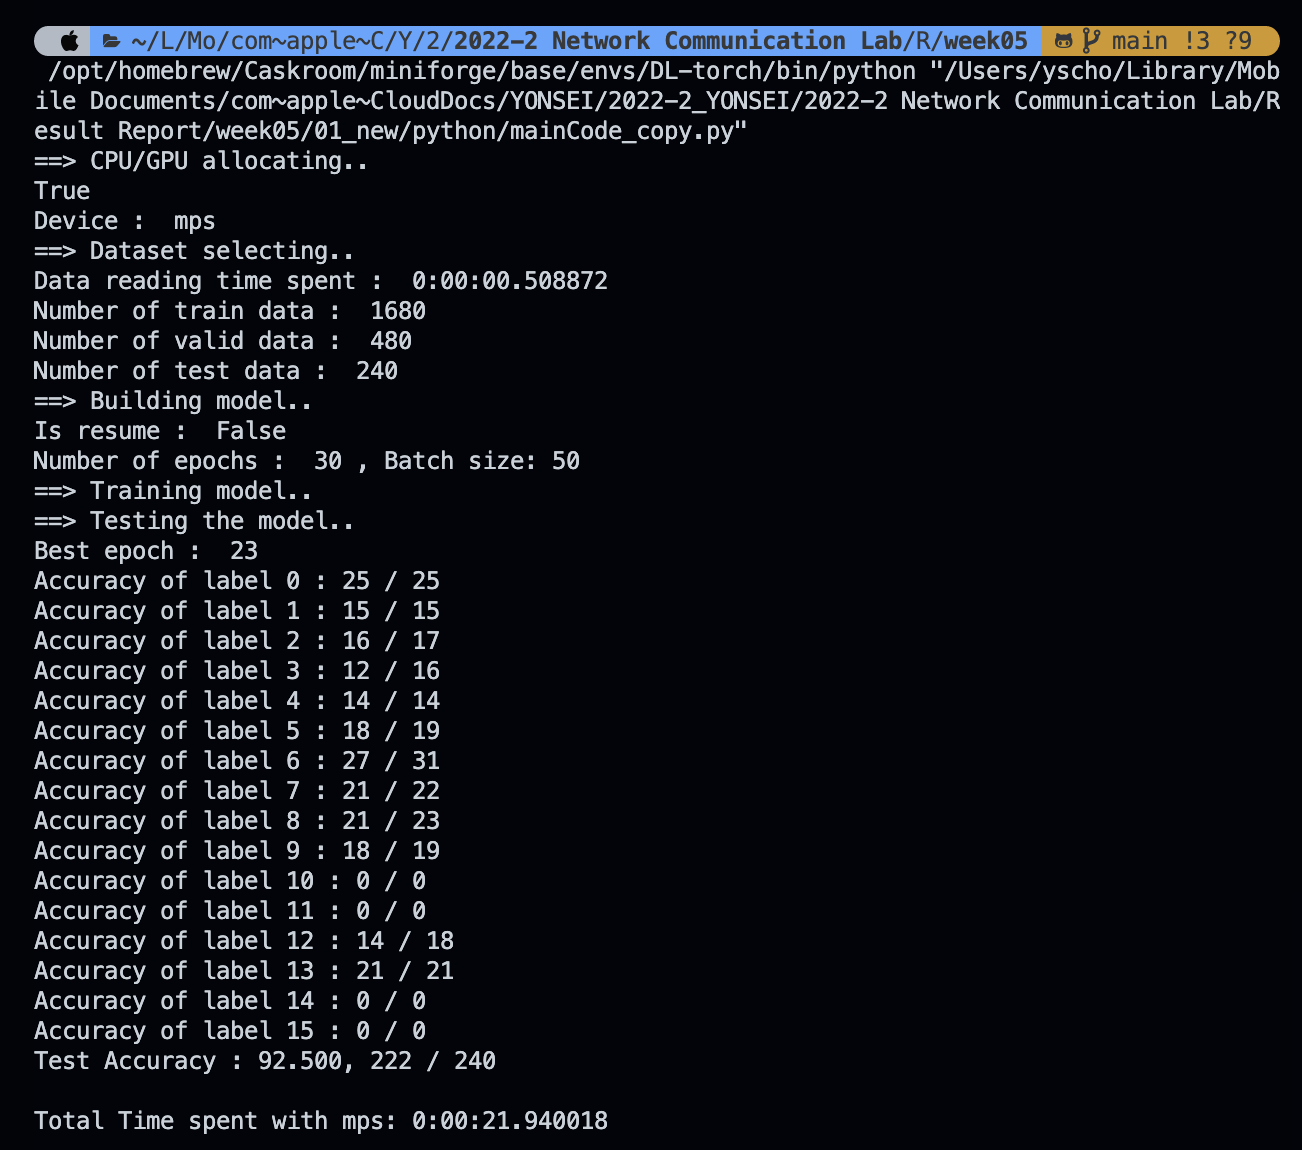
\includegraphics[width=0.48\textwidth]{image/week05/4-2-3.png}
}
\subfloat[Custom Data \& Custom Model , \textbf{Test Accuracy : 98.355}]{
v    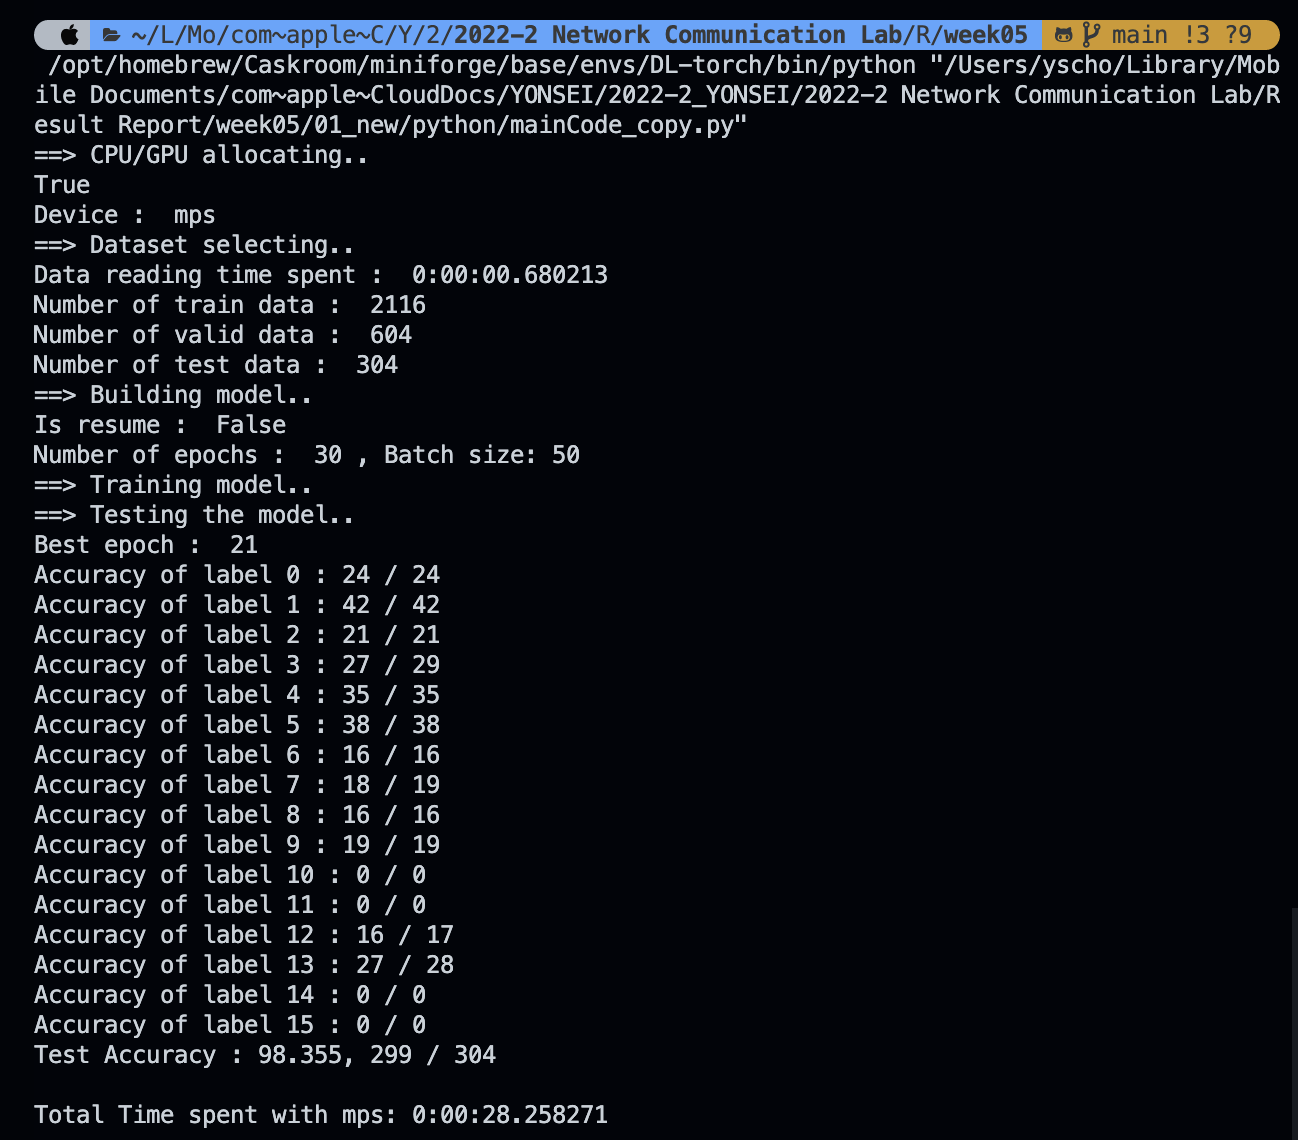
\includegraphics[width=0.48\textwidth]{image/week05/4-2-4.png}
}
\caption{The results of terminal out after the exe the main.py}
\end{figure}

\subsection{Discussion}
In my expereience, as long as the same work that use the simple structure of CNN model apllied in MNIST dataset\footnote{The input size of the minst dataset is $\small 1 \times 28 \times 28$} , that. the addition of the layer makes the accuracy low because of the overfitting problem.

However in this experiment the addition of convolution layer with 3 by 3 filter,We can construct the appropriate model for spectogram dataset to extract an appropriate number of characteristics without overfitting due to the size of the larger input image compared to mnist, the performance of the classifier could be improved.